% Options for packages loaded elsewhere
\PassOptionsToPackage{unicode}{hyperref}
\PassOptionsToPackage{hyphens}{url}
\PassOptionsToPackage{dvipsnames,svgnames,x11names}{xcolor}
%
\documentclass[
  letterpaper,
  DIV=11,
  numbers=noendperiod]{scrartcl}

\usepackage{amsmath,amssymb}
\usepackage{iftex}
\ifPDFTeX
  \usepackage[T1]{fontenc}
  \usepackage[utf8]{inputenc}
  \usepackage{textcomp} % provide euro and other symbols
\else % if luatex or xetex
  \usepackage{unicode-math}
  \defaultfontfeatures{Scale=MatchLowercase}
  \defaultfontfeatures[\rmfamily]{Ligatures=TeX,Scale=1}
\fi
\usepackage{lmodern}
\ifPDFTeX\else  
    % xetex/luatex font selection
\fi
% Use upquote if available, for straight quotes in verbatim environments
\IfFileExists{upquote.sty}{\usepackage{upquote}}{}
\IfFileExists{microtype.sty}{% use microtype if available
  \usepackage[]{microtype}
  \UseMicrotypeSet[protrusion]{basicmath} % disable protrusion for tt fonts
}{}
\makeatletter
\@ifundefined{KOMAClassName}{% if non-KOMA class
  \IfFileExists{parskip.sty}{%
    \usepackage{parskip}
  }{% else
    \setlength{\parindent}{0pt}
    \setlength{\parskip}{6pt plus 2pt minus 1pt}}
}{% if KOMA class
  \KOMAoptions{parskip=half}}
\makeatother
\usepackage{xcolor}
\setlength{\emergencystretch}{3em} % prevent overfull lines
\setcounter{secnumdepth}{-\maxdimen} % remove section numbering
% Make \paragraph and \subparagraph free-standing
\makeatletter
\ifx\paragraph\undefined\else
  \let\oldparagraph\paragraph
  \renewcommand{\paragraph}{
    \@ifstar
      \xxxParagraphStar
      \xxxParagraphNoStar
  }
  \newcommand{\xxxParagraphStar}[1]{\oldparagraph*{#1}\mbox{}}
  \newcommand{\xxxParagraphNoStar}[1]{\oldparagraph{#1}\mbox{}}
\fi
\ifx\subparagraph\undefined\else
  \let\oldsubparagraph\subparagraph
  \renewcommand{\subparagraph}{
    \@ifstar
      \xxxSubParagraphStar
      \xxxSubParagraphNoStar
  }
  \newcommand{\xxxSubParagraphStar}[1]{\oldsubparagraph*{#1}\mbox{}}
  \newcommand{\xxxSubParagraphNoStar}[1]{\oldsubparagraph{#1}\mbox{}}
\fi
\makeatother

\usepackage{color}
\usepackage{fancyvrb}
\newcommand{\VerbBar}{|}
\newcommand{\VERB}{\Verb[commandchars=\\\{\}]}
\DefineVerbatimEnvironment{Highlighting}{Verbatim}{commandchars=\\\{\}}
% Add ',fontsize=\small' for more characters per line
\usepackage{framed}
\definecolor{shadecolor}{RGB}{241,243,245}
\newenvironment{Shaded}{\begin{snugshade}}{\end{snugshade}}
\newcommand{\AlertTok}[1]{\textcolor[rgb]{0.68,0.00,0.00}{#1}}
\newcommand{\AnnotationTok}[1]{\textcolor[rgb]{0.37,0.37,0.37}{#1}}
\newcommand{\AttributeTok}[1]{\textcolor[rgb]{0.40,0.45,0.13}{#1}}
\newcommand{\BaseNTok}[1]{\textcolor[rgb]{0.68,0.00,0.00}{#1}}
\newcommand{\BuiltInTok}[1]{\textcolor[rgb]{0.00,0.23,0.31}{#1}}
\newcommand{\CharTok}[1]{\textcolor[rgb]{0.13,0.47,0.30}{#1}}
\newcommand{\CommentTok}[1]{\textcolor[rgb]{0.37,0.37,0.37}{#1}}
\newcommand{\CommentVarTok}[1]{\textcolor[rgb]{0.37,0.37,0.37}{\textit{#1}}}
\newcommand{\ConstantTok}[1]{\textcolor[rgb]{0.56,0.35,0.01}{#1}}
\newcommand{\ControlFlowTok}[1]{\textcolor[rgb]{0.00,0.23,0.31}{\textbf{#1}}}
\newcommand{\DataTypeTok}[1]{\textcolor[rgb]{0.68,0.00,0.00}{#1}}
\newcommand{\DecValTok}[1]{\textcolor[rgb]{0.68,0.00,0.00}{#1}}
\newcommand{\DocumentationTok}[1]{\textcolor[rgb]{0.37,0.37,0.37}{\textit{#1}}}
\newcommand{\ErrorTok}[1]{\textcolor[rgb]{0.68,0.00,0.00}{#1}}
\newcommand{\ExtensionTok}[1]{\textcolor[rgb]{0.00,0.23,0.31}{#1}}
\newcommand{\FloatTok}[1]{\textcolor[rgb]{0.68,0.00,0.00}{#1}}
\newcommand{\FunctionTok}[1]{\textcolor[rgb]{0.28,0.35,0.67}{#1}}
\newcommand{\ImportTok}[1]{\textcolor[rgb]{0.00,0.46,0.62}{#1}}
\newcommand{\InformationTok}[1]{\textcolor[rgb]{0.37,0.37,0.37}{#1}}
\newcommand{\KeywordTok}[1]{\textcolor[rgb]{0.00,0.23,0.31}{\textbf{#1}}}
\newcommand{\NormalTok}[1]{\textcolor[rgb]{0.00,0.23,0.31}{#1}}
\newcommand{\OperatorTok}[1]{\textcolor[rgb]{0.37,0.37,0.37}{#1}}
\newcommand{\OtherTok}[1]{\textcolor[rgb]{0.00,0.23,0.31}{#1}}
\newcommand{\PreprocessorTok}[1]{\textcolor[rgb]{0.68,0.00,0.00}{#1}}
\newcommand{\RegionMarkerTok}[1]{\textcolor[rgb]{0.00,0.23,0.31}{#1}}
\newcommand{\SpecialCharTok}[1]{\textcolor[rgb]{0.37,0.37,0.37}{#1}}
\newcommand{\SpecialStringTok}[1]{\textcolor[rgb]{0.13,0.47,0.30}{#1}}
\newcommand{\StringTok}[1]{\textcolor[rgb]{0.13,0.47,0.30}{#1}}
\newcommand{\VariableTok}[1]{\textcolor[rgb]{0.07,0.07,0.07}{#1}}
\newcommand{\VerbatimStringTok}[1]{\textcolor[rgb]{0.13,0.47,0.30}{#1}}
\newcommand{\WarningTok}[1]{\textcolor[rgb]{0.37,0.37,0.37}{\textit{#1}}}

\providecommand{\tightlist}{%
  \setlength{\itemsep}{0pt}\setlength{\parskip}{0pt}}\usepackage{longtable,booktabs,array}
\usepackage{calc} % for calculating minipage widths
% Correct order of tables after \paragraph or \subparagraph
\usepackage{etoolbox}
\makeatletter
\patchcmd\longtable{\par}{\if@noskipsec\mbox{}\fi\par}{}{}
\makeatother
% Allow footnotes in longtable head/foot
\IfFileExists{footnotehyper.sty}{\usepackage{footnotehyper}}{\usepackage{footnote}}
\makesavenoteenv{longtable}
\usepackage{graphicx}
\makeatletter
\newsavebox\pandoc@box
\newcommand*\pandocbounded[1]{% scales image to fit in text height/width
  \sbox\pandoc@box{#1}%
  \Gscale@div\@tempa{\textheight}{\dimexpr\ht\pandoc@box+\dp\pandoc@box\relax}%
  \Gscale@div\@tempb{\linewidth}{\wd\pandoc@box}%
  \ifdim\@tempb\p@<\@tempa\p@\let\@tempa\@tempb\fi% select the smaller of both
  \ifdim\@tempa\p@<\p@\scalebox{\@tempa}{\usebox\pandoc@box}%
  \else\usebox{\pandoc@box}%
  \fi%
}
% Set default figure placement to htbp
\def\fps@figure{htbp}
\makeatother

\KOMAoption{captions}{tableheading}
\makeatletter
\@ifpackageloaded{caption}{}{\usepackage{caption}}
\AtBeginDocument{%
\ifdefined\contentsname
  \renewcommand*\contentsname{Table of contents}
\else
  \newcommand\contentsname{Table of contents}
\fi
\ifdefined\listfigurename
  \renewcommand*\listfigurename{List of Figures}
\else
  \newcommand\listfigurename{List of Figures}
\fi
\ifdefined\listtablename
  \renewcommand*\listtablename{List of Tables}
\else
  \newcommand\listtablename{List of Tables}
\fi
\ifdefined\figurename
  \renewcommand*\figurename{Figure}
\else
  \newcommand\figurename{Figure}
\fi
\ifdefined\tablename
  \renewcommand*\tablename{Table}
\else
  \newcommand\tablename{Table}
\fi
}
\@ifpackageloaded{float}{}{\usepackage{float}}
\floatstyle{ruled}
\@ifundefined{c@chapter}{\newfloat{codelisting}{h}{lop}}{\newfloat{codelisting}{h}{lop}[chapter]}
\floatname{codelisting}{Listing}
\newcommand*\listoflistings{\listof{codelisting}{List of Listings}}
\makeatother
\makeatletter
\makeatother
\makeatletter
\@ifpackageloaded{caption}{}{\usepackage{caption}}
\@ifpackageloaded{subcaption}{}{\usepackage{subcaption}}
\makeatother

\usepackage{bookmark}

\IfFileExists{xurl.sty}{\usepackage{xurl}}{} % add URL line breaks if available
\urlstyle{same} % disable monospaced font for URLs
\hypersetup{
  pdftitle={Project\_251},
  pdfauthor={Brandon Upper, Ben Murdock, Hannah Lyons},
  colorlinks=true,
  linkcolor={blue},
  filecolor={Maroon},
  citecolor={Blue},
  urlcolor={Blue},
  pdfcreator={LaTeX via pandoc}}


\title{Project\_251}
\author{Brandon Upper, Ben Murdock, Hannah Lyons}
\date{}

\begin{document}
\maketitle


\begin{Shaded}
\begin{Highlighting}[]
\CommentTok{\#library}
\FunctionTok{library}\NormalTok{(vroom)}
\FunctionTok{library}\NormalTok{(ggplot2)}
\FunctionTok{library}\NormalTok{(tidyverse)}
\end{Highlighting}
\end{Shaded}

\begin{verbatim}
-- Attaching core tidyverse packages ------------------------ tidyverse 2.0.0 --
v dplyr     1.1.4     v readr     2.1.5
v forcats   1.0.0     v stringr   1.5.2
v lubridate 1.9.4     v tibble    3.3.0
v purrr     1.1.0     v tidyr     1.3.1
-- Conflicts ------------------------------------------ tidyverse_conflicts() --
x readr::col_character()   masks vroom::col_character()
x readr::col_date()        masks vroom::col_date()
x readr::col_datetime()    masks vroom::col_datetime()
x readr::col_double()      masks vroom::col_double()
x readr::col_factor()      masks vroom::col_factor()
x readr::col_guess()       masks vroom::col_guess()
x readr::col_integer()     masks vroom::col_integer()
x readr::col_logical()     masks vroom::col_logical()
x readr::col_number()      masks vroom::col_number()
x readr::col_skip()        masks vroom::col_skip()
x readr::col_time()        masks vroom::col_time()
x readr::cols()            masks vroom::cols()
x readr::date_names_lang() masks vroom::date_names_lang()
x readr::default_locale()  masks vroom::default_locale()
x dplyr::filter()          masks stats::filter()
x readr::fwf_cols()        masks vroom::fwf_cols()
x readr::fwf_empty()       masks vroom::fwf_empty()
x readr::fwf_positions()   masks vroom::fwf_positions()
x readr::fwf_widths()      masks vroom::fwf_widths()
x dplyr::lag()             masks stats::lag()
x readr::locale()          masks vroom::locale()
x readr::output_column()   masks vroom::output_column()
x readr::problems()        masks vroom::problems()
i Use the conflicted package (<http://conflicted.r-lib.org/>) to force all conflicts to become errors
\end{verbatim}

\begin{Shaded}
\begin{Highlighting}[]
\FunctionTok{library}\NormalTok{(dplyr)}
\end{Highlighting}
\end{Shaded}

\begin{Shaded}
\begin{Highlighting}[]
\CommentTok{\#data}
\NormalTok{shootouts }\OtherTok{\textless{}{-}} \FunctionTok{vroom}\NormalTok{(}\StringTok{\textquotesingle{}./WorldCupShootouts.csv\textquotesingle{}}\NormalTok{)}
\end{Highlighting}
\end{Shaded}

\begin{verbatim}
Rows: 304 Columns: 9
-- Column specification --------------------------------------------------------
Delimiter: ","
chr (3): Team, Foot, Keeper
dbl (6): Game_id, Zone, OnTarget, Goal, Penalty_Number, Elimination

i Use `spec()` to retrieve the full column specification for this data.
i Specify the column types or set `show_col_types = FALSE` to quiet this message.
\end{verbatim}

\#Short Written Description Our dataset contains information on World
Cup penalty shootouts from Spain 1982 to Russia 2018 sourced from
Kaggle. URL:
\href{https://www.kaggle.com/datasets/pablollanderos33/world-cup-penalty-shootouts}{World
Cup Penalty Shootouts Dataset}

The dataset contains 305 rows in total. The first row is a descriptive
header, leaving 304 rows of actual data and 9 columns. The columns
include: Game\_id: Each team in a single game get's a number. Numbers
are not repeated across separate games. Team: The country team of the
kicker. Zone: The goal was divided into 9 sections, each labeled by
number. This number is the zone. Foot: The foot used to take the shot
(Left/Right). Keeper: The direction the goalkeeper dove(Left/Right) On
Target: Indicates whether the shot would have been a goal if the keeper
had not intervened(1 = Yes, 0 = No) Goal: Whether the penalty was
successfully scored (1 = Goal, 0 = Miss) Penalty number: The order of
the penalty within the shootout Elimination: Indicates whether the
penalty could end the game (1 = Yes, 0 = No)

\section{Ben: Proposed Research Question, left/right success bar
graph.}\label{ben-proposed-research-question-leftright-success-bar-graph.}

We would like to determine if there is a difference between proportion
of successful penalty kicks of right footed vs.~left footed soccer
players.

\section{Brandon: EDA}\label{brandon-eda}

The proposed data source and a well-organized and well-articulated
exploratory analysis of its contents (this should include well-labeled
plots created in R).

Libraries

\begin{Shaded}
\begin{Highlighting}[]
\FunctionTok{library}\NormalTok{(ggplot2)}
\FunctionTok{library}\NormalTok{(vroom)}
\FunctionTok{library}\NormalTok{(tidyverse)}
\end{Highlighting}
\end{Shaded}

Read File

\begin{Shaded}
\begin{Highlighting}[]
\NormalTok{Soccer\_data }\OtherTok{\textless{}{-}} \FunctionTok{vroom}\NormalTok{(}\StringTok{"WorldCupShootouts.csv"}\NormalTok{)}
\end{Highlighting}
\end{Shaded}

\begin{verbatim}
Rows: 304 Columns: 9
-- Column specification --------------------------------------------------------
Delimiter: ","
chr (3): Team, Foot, Keeper
dbl (6): Game_id, Zone, OnTarget, Goal, Penalty_Number, Elimination

i Use `spec()` to retrieve the full column specification for this data.
i Specify the column types or set `show_col_types = FALSE` to quiet this message.
\end{verbatim}

\begin{Shaded}
\begin{Highlighting}[]
\FunctionTok{summary}\NormalTok{(Soccer\_data)}
\end{Highlighting}
\end{Shaded}

\begin{verbatim}
    Game_id          Team                Zone           Foot          
 Min.   : 1.00   Length:304         Min.   :1.000   Length:304        
 1st Qu.: 8.00   Class :character   1st Qu.:4.000   Class :character  
 Median :15.00   Mode  :character   Median :6.000   Mode  :character  
 Mean   :15.37                      Mean   :5.595                     
 3rd Qu.:23.00                      3rd Qu.:7.000                     
 Max.   :30.00                      Max.   :9.000                     
                                    NA's   :25                        
    Keeper             OnTarget           Goal        Penalty_Number  
 Length:304         Min.   :0.0000   Min.   :0.0000   Min.   : 1.000  
 Class :character   1st Qu.:1.0000   1st Qu.:0.0000   1st Qu.: 3.000  
 Mode  :character   Median :1.0000   Median :1.0000   Median : 6.000  
                    Mean   :0.9176   Mean   :0.6989   Mean   : 5.579  
                    3rd Qu.:1.0000   3rd Qu.:1.0000   3rd Qu.: 8.000  
                    Max.   :1.0000   Max.   :1.0000   Max.   :12.000  
                    NA's   :25       NA's   :25                       
  Elimination    
 Min.   :0.0000  
 1st Qu.:0.0000  
 Median :0.0000  
 Mean   :0.1286  
 3rd Qu.:0.0000  
 Max.   :1.0000  
 NA's   :24      
\end{verbatim}

\begin{Shaded}
\begin{Highlighting}[]
\FunctionTok{head}\NormalTok{(Soccer\_data)}
\end{Highlighting}
\end{Shaded}

\begin{verbatim}
# A tibble: 6 x 9
  Game_id Team   Zone Foot  Keeper OnTarget  Goal Penalty_Number Elimination
    <dbl> <chr> <dbl> <chr> <chr>     <dbl> <dbl>          <dbl>       <dbl>
1       1 FRA       7 R     R             1     1              1           0
2       1 GER       9 R     C             1     1              2           0
3       1 FRA       6 R     L             1     1              3           0
4       1 GER       2 R     C             1     1              4           0
5       1 FRA       9 R     L             1     1              5           0
6       1 GER       4 R     L             1     0              6           0
\end{verbatim}

Reading in our file we can see various factors, features and variables
that are described more in depth in the above short description of the
data. From this code we can see the first five rows of the data and
notice that many points are read in as doubles and characters. For the
final analysis, we likely will convert some of these variables for
simplicity

Basic plots about Goals and Penalties

\begin{Shaded}
\begin{Highlighting}[]
\NormalTok{Soccer\_data }\OtherTok{\textless{}{-}}\NormalTok{ Soccer\_data }\SpecialCharTok{\%\textgreater{}\%}
  \FunctionTok{filter}\NormalTok{(}\FunctionTok{is.finite}\NormalTok{(Zone)) }
\FunctionTok{ggplot}\NormalTok{(}\AttributeTok{data =}\NormalTok{ Soccer\_data) }\SpecialCharTok{+} 
  \FunctionTok{geom\_bar}\NormalTok{(}\AttributeTok{mapping =} \FunctionTok{aes}\NormalTok{(}\AttributeTok{x =}\NormalTok{ Zone), }
           \AttributeTok{fill =} \StringTok{"lightblue"}\NormalTok{) }\SpecialCharTok{+} \FunctionTok{ggtitle}\NormalTok{(}\StringTok{"Goals by Zone"}\NormalTok{) }\SpecialCharTok{+} \FunctionTok{ylab}\NormalTok{(}\StringTok{"Count"}\NormalTok{)}
\end{Highlighting}
\end{Shaded}

\pandocbounded{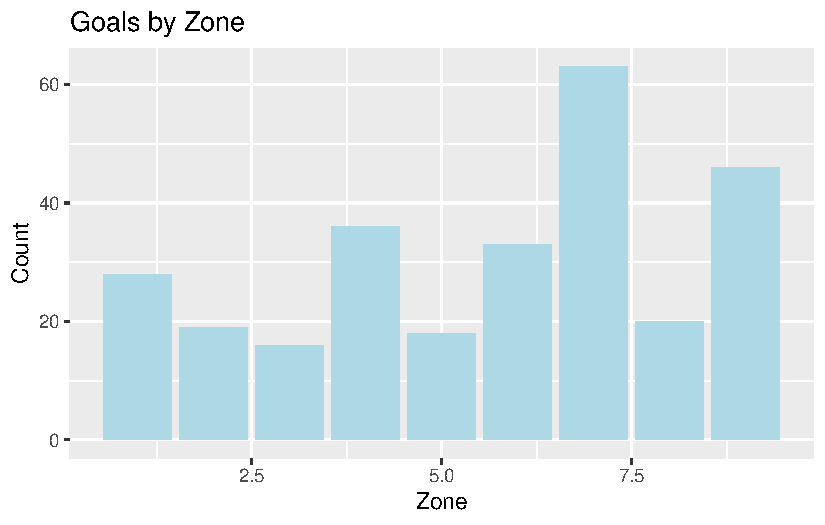
\includegraphics[keepaspectratio]{Project_251_files/figure-pdf/unnamed-chunk-5-1.pdf}}

\begin{Shaded}
\begin{Highlighting}[]
\FunctionTok{ggplot}\NormalTok{(}\AttributeTok{data =}\NormalTok{ Soccer\_data) }\SpecialCharTok{+} 
  \FunctionTok{geom\_bar}\NormalTok{(}\AttributeTok{mapping =} \FunctionTok{aes}\NormalTok{(}\AttributeTok{y =}\NormalTok{ Penalty\_Number), }\AttributeTok{fill =} \StringTok{"navyblue"}\NormalTok{) }\SpecialCharTok{+} 
  \FunctionTok{ggtitle}\NormalTok{(}\StringTok{"Penalty Number by Count"}\NormalTok{) }\SpecialCharTok{+} \FunctionTok{ylab}\NormalTok{(}\StringTok{"Penalty Number"}\NormalTok{) }\SpecialCharTok{+} \FunctionTok{xlab}\NormalTok{(}\StringTok{"Count"}\NormalTok{)}
\end{Highlighting}
\end{Shaded}

\pandocbounded{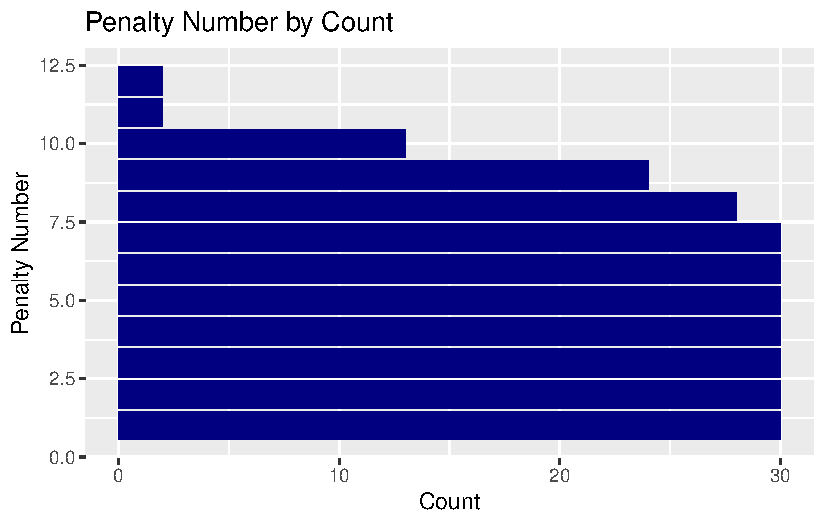
\includegraphics[keepaspectratio]{Project_251_files/figure-pdf/unnamed-chunk-5-2.pdf}}

These graphs give some visuals to some of the data and the types
penalties we're seeing. For example, its clear that different zones have
higher portions of goals scored, and when we recognize that the zone
targeted and thereby goal likelihood can be highly influenced by right
vs left footed kickers. From prior soccer experience, we could look for
tendencies in the final project for kickers to shoot towards met
opposite of their dominant foot. The second graph also displays how long
the shootout lasts for, and its clear that most of them end before or
around the twelfth number.

Looking for Correlation

\begin{Shaded}
\begin{Highlighting}[]
\NormalTok{numeric\_data }\OtherTok{\textless{}{-}}\NormalTok{ Soccer\_data }\SpecialCharTok{\%\textgreater{}\%}
  \FunctionTok{select}\NormalTok{(}\FunctionTok{where}\NormalTok{(is.numeric))}

\FunctionTok{library}\NormalTok{(corrplot)}
\end{Highlighting}
\end{Shaded}

\begin{verbatim}
corrplot 0.95 loaded
\end{verbatim}

\begin{Shaded}
\begin{Highlighting}[]
\NormalTok{cor\_matrix }\OtherTok{\textless{}{-}} \FunctionTok{cor}\NormalTok{(numeric\_data)}
\FunctionTok{corrplot}\NormalTok{(cor\_matrix)}
\end{Highlighting}
\end{Shaded}

\pandocbounded{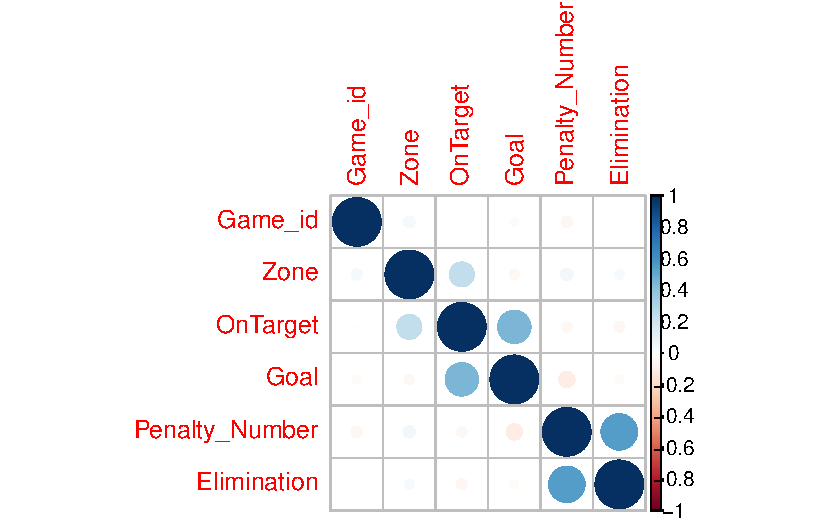
\includegraphics[keepaspectratio]{Project_251_files/figure-pdf/unnamed-chunk-6-1.pdf}}

There seems to be no strong correlations between any of the numeric
variables. This is useful as we can see that this data is unlikely to
have issues with multicollinearity.

\begin{Shaded}
\begin{Highlighting}[]
\CommentTok{\#left vs right foot {-} success proportion}

\NormalTok{plot\_data }\OtherTok{\textless{}{-}}\NormalTok{ Soccer\_data }\SpecialCharTok{\%\textgreater{}\%}
  \FunctionTok{select}\NormalTok{(Foot, Goal) }\SpecialCharTok{\%\textgreater{}\%} 
  \FunctionTok{filter}\NormalTok{(Foot }\SpecialCharTok{\%in\%} \FunctionTok{c}\NormalTok{(}\StringTok{"L"}\NormalTok{, }\StringTok{"R"}\NormalTok{),}
\NormalTok{         Goal }\SpecialCharTok{\%in\%} \FunctionTok{c}\NormalTok{(}\DecValTok{0}\NormalTok{, }\DecValTok{1}\NormalTok{)) }\SpecialCharTok{\%\textgreater{}\%}
  \FunctionTok{mutate}\NormalTok{(}\AttributeTok{Goal\_Status =} \FunctionTok{factor}\NormalTok{(Goal, }
                              \AttributeTok{levels =} \FunctionTok{c}\NormalTok{(}\DecValTok{0}\NormalTok{, }\DecValTok{1}\NormalTok{), }
                              \AttributeTok{labels =} \FunctionTok{c}\NormalTok{(}\StringTok{"Miss"}\NormalTok{, }\StringTok{"Success"}\NormalTok{)))}

\FunctionTok{ggplot}\NormalTok{(plot\_data, }\FunctionTok{aes}\NormalTok{(}\AttributeTok{x =}\NormalTok{ Foot, }\AttributeTok{fill =}\NormalTok{ Goal\_Status)) }\SpecialCharTok{+}
  \FunctionTok{geom\_bar}\NormalTok{(}\AttributeTok{position =} \StringTok{"dodge"}\NormalTok{)}
\end{Highlighting}
\end{Shaded}

\pandocbounded{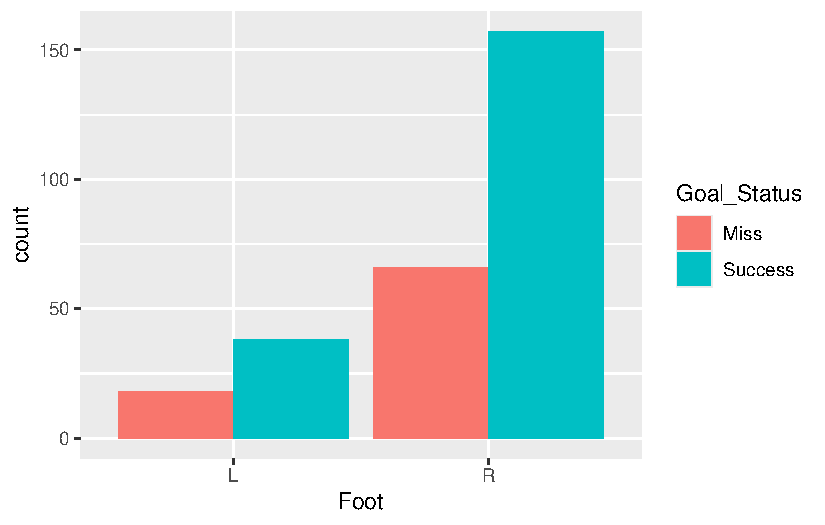
\includegraphics[keepaspectratio]{Project_251_files/figure-pdf/unnamed-chunk-7-1.pdf}}




\end{document}
